\documentclass{ctexart}
\usepackage{geometry}
\usepackage{diagbox}
\usepackage{graphicx}
\usepackage{subfigure}
\usepackage{amsmath}
\usepackage{amssymb}
\usepackage{indentfirst}
\usepackage{xfrac}
\usepackage{color}
\usepackage[table]{xcolor}
\usepackage{multirow}
\usepackage{titlesec}
\usepackage{bm}
\usepackage{caption}
\usepackage{booktabs}
\usepackage{ulem}
\usepackage{float}
% 调节页边距
\geometry{a4paper,left=3cm,right=3cm,top=3cm,bottom=3cm}
\renewcommand{\abstractname}{\large 摘要\\}
\title{UP主粉丝数的影响因素分析}
\author{CDA小组}
\date{}
\begin{document}
\maketitle
%------------------------------------摘要------------------------------------
\begin{abstract}
    这里是摘要
\end{abstract}
%------------------------------------目录------------------------------------
\tableofcontents
%------------------------------------正文------------------------------------
\newpage
\section{背景介绍}
Bilibili视频网站(下文简称B站)在近年愈发受到年轻人的欢迎,数量庞大的UP主群体为B站的视频生态的多样性做出了
非常大的贡献。在庞大的UP主群体之下,UP主的粉丝数也有显著的差异。本研究旨在通过研究各种影响因素与UP主的粉丝
数量的分层不同带来的影响。\\
\indent 本次研究的数据来源于ifans网站,网站上提供了粉丝量、最近更新时间、分区、视频数、
充电数、近8篇平均视频投币数、近8篇平均视频弹幕数、近8篇平均视频收藏数、近8篇平均视频点赞数、
近8篇平均视频播放数、近8篇平均视频评论数、近8篇平均视频分享数数据、性别数据,本研究将所有变量均放入模型中进行研究,
同时研究是否能够有减少变量的方法。本研究凭借网站上的粉丝数量分区,
将粉丝量的分区分为“<10万”,“10万~50万”,“50万~100万”,“>100万”四个分区,作为后续分类型数据分析的基础。\\
\indent 由于不同分区的UP主人数差异较大,本研究采用回溯性研究方法,即在四个粉丝量的分区分别抽取250个UP主的数据
进行研究分析。
\section{数据预处理}
由于每个变量的单位相差较大,为了避免单位造成的影响,本研究将所有非分类型数据进行归一化处理。
由于选择的解释变量均为非负数据,为保持这一性质,采用以下的归一化方法。
\begin{equation}
    \tilde{x} = \frac{x-\alpha}{\beta - \alpha}
\end{equation}
其中$\alpha$,$\beta$分别为本解释变量中的最大值与最小值。
\section{探索性数据分析}
\subsection{数据可视化}
首先,作出各类数据之间相关系数的热量图:
\begin{figure}[htbp]
    \centering
    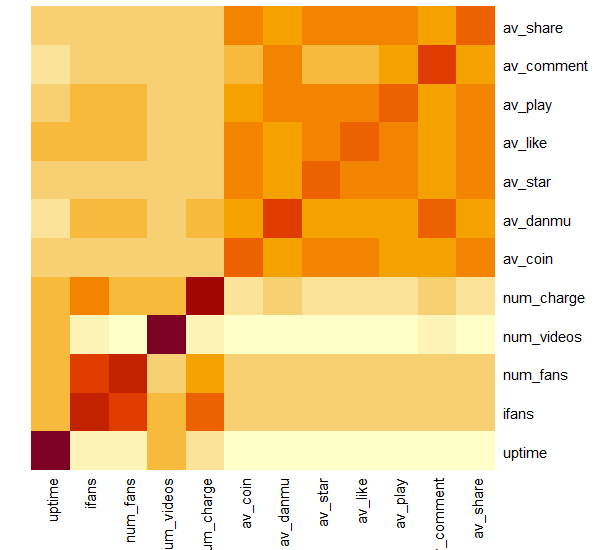
\includegraphics[width=0.40\textwidth]{EDA/Heatmap.png}
    \caption{Heatmap for Correlation}
\end{figure}\\
\indent 由热量图可见,右上角各种平均的线性相关性较强。由于作出Scatter Plot Matrix时,如果变量过多,则容易显示不清楚,因此
选择近8篇平均投币数和近8篇平均点赞数作为各种平均的代表绘制Scatter Plot Matrix。
\begin{figure}[htbp]
    \centering
    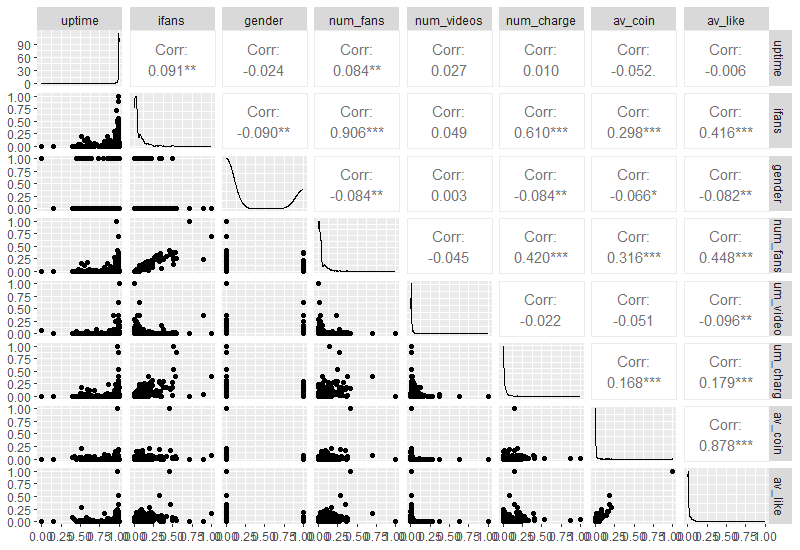
\includegraphics[width=0.60\textwidth]{EDA/Spm.png}
    \caption{Scatter Plot Matrix}
\end{figure}\\
\indent 由Scatter Plot Matrix可见,各类数据间普遍具有一定的相关性,这说明对这些数据建立模型进行分析应该会有一定的效果。同时,由每个变量的核密度
估计可见,各个解释变量是明显右偏的,这说明B站的UP主存在一定的少部分UP主占据了极大的资源的效应。\\
\indent 通过Scatter Plot Matrix,作出两大分区变量粉丝量与性别和与这两个因素有显著作用的的变量之间的箱型图,观察这些因素对
两大分类型变量的影响。
\begin{figure}[htbp]
    \centering
    \begin{minipage}[t]{0.48\textwidth}
        \centering
        \includegraphics[width=\textwidth]{EDA/av_like_gender_boxplot.png}
        \caption{各性别平均点赞数}
    \end{minipage}
    \begin{minipage}[t]{0.48\textwidth}
        \centering
        \includegraphics[width=\textwidth]{EDA/num_charges_gender_boxplot.png}
        \caption{各性别充电数}
    \end{minipage}
\end{figure}
\begin{figure}[htbp]
    \centering
    \begin{minipage}[t]{0.48\textwidth}
        \centering
        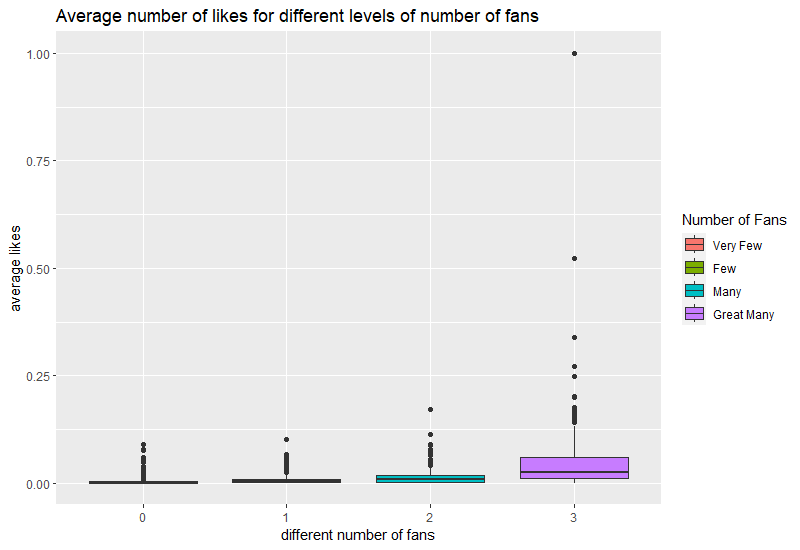
\includegraphics[width=\textwidth]{EDA/av_like_fans_boxplot.png}
        \caption{各粉丝量平均点赞数}
    \end{minipage}
    \begin{minipage}[t]{0.48\textwidth}
        \centering
        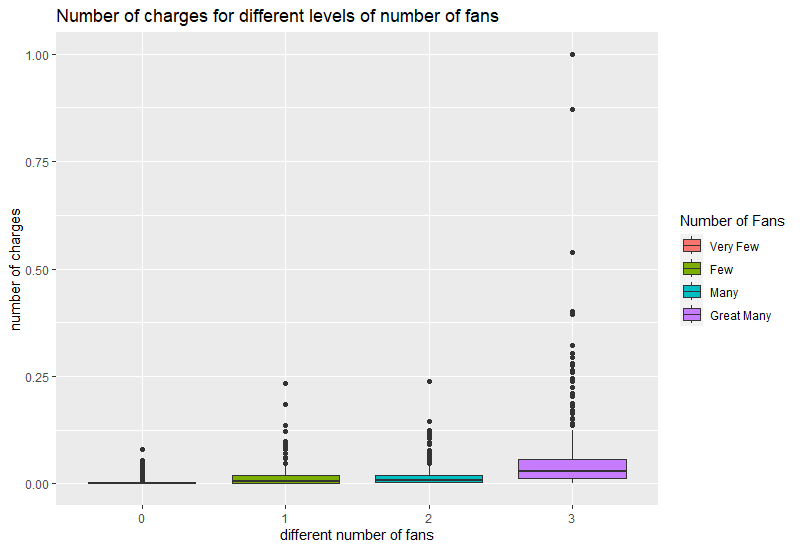
\includegraphics[width=\textwidth]{EDA/num_charge_fan_boxplot.png}
        \caption{各粉丝量充电数}
    \end{minipage}
\end{figure}\\
\indent 由图可见,对于部分解释变量,其对不同性别确实有显著的影响;对于平均点赞数和充电数而言,均表现为男性的
离群值点远大于女性的特点。而诸多解释变量对于粉丝量也有显著的作用,与上述分析相似的,对于粉丝量较少的三类,实际上
两个变量的表现较为相似,而粉丝量大于100万的样本,在点赞量和充电数上,无论是平均值还是数量高的值都明显多于前三类。
这映照了之前认为的少部分UP主获得了最多的关注的同时,也按时是否需要优化分区结构,能够获得更好的效果。\\
\\
\indent 由于解释变量仍较多,并且从Scatter Plot Matrix可以看出部分解释变量之间存在较为显著的线性相关性,
因此考虑是否能对解释变量进行一定程度的筛选。下面考虑利用主成分分析(PCA)和LASSO两种方法对是否能够减少解释变量数量进行分析。
\subsection{主成分分析}
对归一化后的连续型解释变量进行主成分分析,所得肘图如下图:
\begin{figure}[htbp]
    \centering
    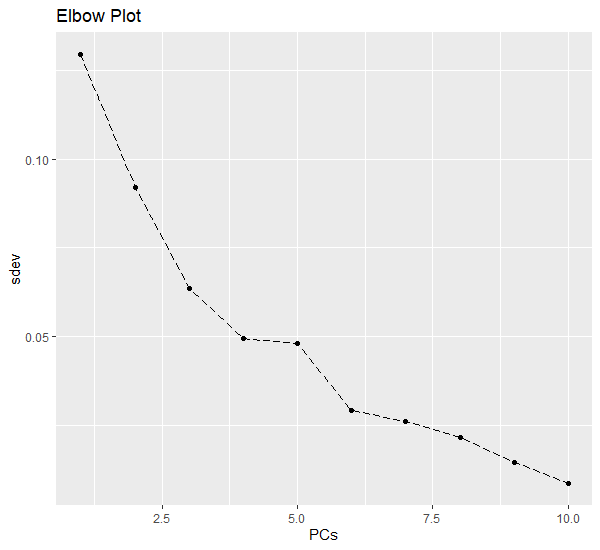
\includegraphics[width=0.45\textwidth]{EDA/PCA_elbow.png}
    \caption{PCA肘图}
\end{figure}\\
\indent 由肘图可见,实际上PCA的效果并不好,在拐点后方程下降速度仍较为显著,
并且拐点处的方差仍较大。如果要保留99\%的信息量,则可舍弃最后两个主成分;如果要保留95\%的信息量,则可舍弃最后四个主成分。一定程度上起到了降维
的效果。PCA的旋转矩阵如下表:
\begin{table}[htbp]
    \centering
    \begin{tabular}{|c|c|c|c|c|c|c|c|c|c|c|}
    \hline
            & PC1   & PC2   & PC3   & PC4   & PC5   & PC6   & PC7   & PC8   & PC9   & PC10  \\ \hline
    uptime  & -0.17 & 0.97  & 0     & 0.11  & -0.08 & 0.04  & -0.03 & 0.01  & -0.02 & -0.01 \\ \hline
    videos  & -0.04 & 0     & -0.03 & 0.55  & 0.83  & -0.04 & -0.04 & 0     & -0.01 & 0.01  \\ \hline
    charge  & 0.15  & 0.07  & -0.93 & -0.29 & 0.17  & 0.04  & -0.01 & 0     & -0.01 & 0     \\ \hline
    coin    & 0.23  & 0.07  & 0.08  & -0.07 & 0.1   & 0.21  & 0.46  & -0.36 & 0.33  & -0.65 \\ \hline
    danmu   & 0.51  & 0.01  & -0.17 & 0.57  & -0.35 & -0.19 & 0.37  & 0.3   & -0.01 & 0.08  \\ \hline
    star    & 0.3   & 0.08  & 0.16  & -0.2  & 0.16  & 0.09  & 0.31  & -0.26 & -0.78 & 0.17  \\ \hline
    like    & 0.32  & 0.12  & 0.14  & -0.19 & 0.14  & -0.13 & 0.09  & -0.32 & 0.51  & 0.65  \\ \hline
    play    & 0.48  & 0.12  & 0.14  & -0.19 & 0.11  & -0.58 & -0.47 & 0.06  & -0.05 & -0.35 \\ \hline
    comment & 0.31  & -0.03 & -0.07 & 0.33  & -0.21 & 0.49  & -0.56 & -0.44 & -0.05 & 0.01  \\ \hline
    share   & 0.34  & 0.08  & 0.2   & -0.23 & 0.2   & 0.56  & -0.07 & 0.65  & 0.1   & 0.03  \\ \hline
    \end{tabular}
    \caption{PCA旋转矩阵}
\end{table}\\
\indent 由旋转矩阵可见,实际上PCA的解释性较差。又由于本研究主要为解释性研究,因此如果采用PCA后的主成分进行分析,
最后会导致解释性较差,所以将舍弃PCA部分的结果。
\subsection{LASSO}
利用LASSO将所有解释变量放入模型中,分别对粉丝量(分类型)作多分类变量逻辑回归与对粉丝量(连续型)作广义线性回归,得到
均方误差随正则项的变化分别如下两图。
\begin{figure}[htbp]
    \begin{minipage}[t]{0.48\textwidth}
        \centering
        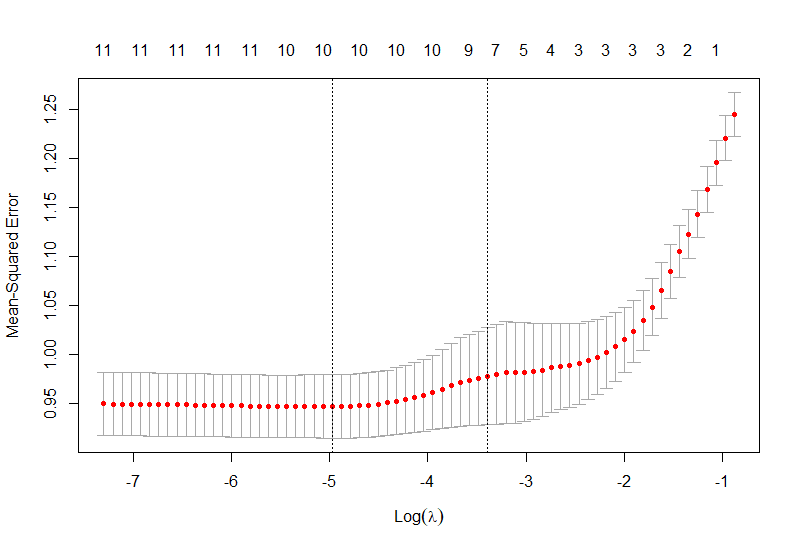
\includegraphics[width=\textwidth]{EDA/lasso_multinomial.png}
        \caption{多分类逻辑回归}
    \end{minipage}
    \begin{minipage}[t]{0.48\textwidth}
        \centering
        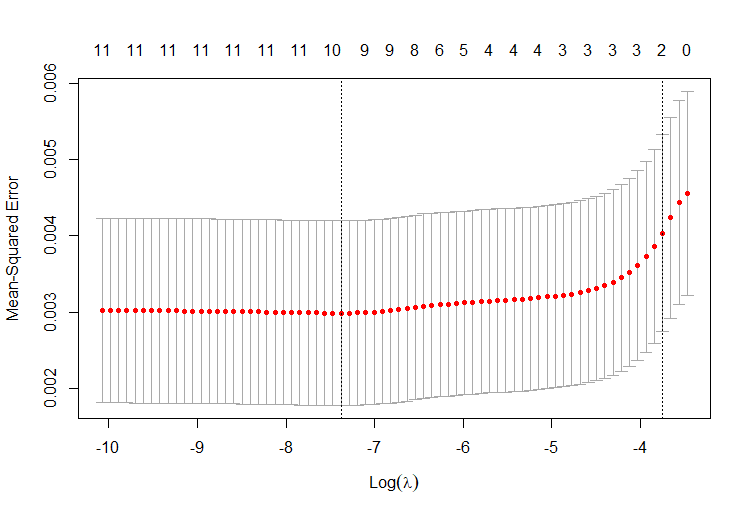
\includegraphics[width=\textwidth]{EDA/lasso_continuous.png}
        \caption{连续型线性回归}
    \end{minipage}
\end{figure}\\
\indent 所得在让均方误差最小的正则项系数与在1个标准差意义下的正则项系数如下表,其中进行多分类逻辑回归得到4个返回的$\lambda$值,
筛选出效果较好的值对应的系数:
\begin{table}[htbp]
    \centering
    \begin{tabular}{ccccc}
    \hline
    \multirow{2}{*}{Name} & \multicolumn{2}{c}{Multinomial} & \multicolumn{2}{c}{Continuous} \\ \cline{2-5} 
                          & min            & 1se            & min            & 1se           \\ \hline
    Intercept             & 8.76           & 5.26           & -0.03          & 0.04          \\
    uptime                & -8.16          & -5.69          & 0.05           & 0             \\
    gender                & 0.08           & 0.15           & 0              & 0             \\
    videos                & -1.08          & 0              & 0              & 0             \\
    charge                & -54.93         & -20.74         & 0.34           & 0.05          \\
    coin                  & 0              & 0              & -0.3           & 0             \\
    danmu                 & 0              & 0              & 0.09           & 0             \\
    star                  & 8.08           & 0              & -0.11          & 0             \\
    like                  & -73.91         & -21.17         & 0.66           & 0             \\
    play                  & -13.79         & 0              & 0.2            & 0.1           \\
    comment               & -1.07          & 0              & -0.06          & 0             \\
    share                 & 22.47          & 0              & -0.16          & 0             \\ \hline
    \end{tabular}
    \caption{正则后系数表}
\end{table}\\
\indent 由上表可见,使用LASSO多类别逻辑回归和线性回归得到的系数有较为明显的区别,因此说明经过将粉丝量分类,得到了
不同的回归结果,有不同的解释效应。因此,在进行多分类逻辑回归会得到直接线性回归不同的结果。由于两个1个标准差内的结果
都省略了过多的变量,可能造成解释能力不足,因此在进行多分类逻辑回归时,考虑舍弃投币数和弹幕数两个变量。


\section{多分类逻辑回归分析}

为了分析性别以及点赞数、充电数这些连续型变量与up主粉丝数分区的关系,我们采用多分类
逻辑回归模型进行建模分析。

\subsection{变量选取}

根据前面部分可知,我们按照“<10万”,“10万~50万”,“50万~100万”,“>100万”的标准将up
主按照粉丝数分成了4类,我们将这4个up主量级分别记为小up主,中up主,大up主和超级up主,
得到响应变量如下:
\begin{table}[H]
    \centering
    \begin{tabular}{ccc}
        \toprule
         响应变量 & 变量类型 & 变量含义  \\
        \midrule
         fans\_cat & Multicategory & 粉丝数的分类,small, middle, big, super big四类 \\
        \bottomrule
    \end{tabular}
    \caption{多分类逻辑回归响应变量}
\end{table}

对于解释变量,我们一共有1个二分类的性别变量和9个归一化后的连续型变量,各个
变量的含义如下标所示,根据LASSO部分的分析,我们可以去掉av\_coin和av\_danmu两个变量,
选择余下8个解释变量作为建模最初的8个变量。

\begin{table}[H]
    \centering
    \begin{tabular}{ccc}
        \toprule
          解释变量 & 变量类型 & 变量含义  \\
        \midrule
          gender & binary & 性别, 1代表女性, 0代表男性 \\
          num\_videos & continuous & 视频数的多少, 单位为个\\
          num\_charge & continuous & 充电数的多少, 单位为个\\
          av\_star & continuous & 最近8个视频的平均收藏量, 单位为个\\
          av\_like & continuous & 最近8个视频的平均点赞数, 单位为个\\
          av\_play & continuous & 最近8个视频的平均播放数, 单位为次\\
          av\_comment & continuous & 最近8个视频的平均评论数, 单位为个\\
          av\_share & continuous & 最近8个视频的平均分享数, 单位为个\\
          \sout{av\_coin} & continuous & 最近8个视频的平均投币量, 单位为个\\
          \sout{av\_danmu} & continuous & 最近8个视频的平均弹幕数量, 单位为个\\
        \bottomrule
     \end{tabular}
    \caption{多分类逻辑回归解释变量}
\end{table}

为初步地观察解释变量与up主粉丝数分类的关系,我们在四个分类中各随机抽取75个up主,绘
制出这300个up主的并行坐标图如下图所示,图中每一条线就是一个up主在各解释变量的坐标,up主的粉
丝数分类由线的颜色和线型表示。从图中我们可以看出超级up主的充电数,近期视频的充电数、
平均点赞数、播放量和评论数都趋向于最大,而有一些小up主的近期平均收藏量在抽取的up主
中可以达到最大。

\begin{figure}[H]
    \centering
    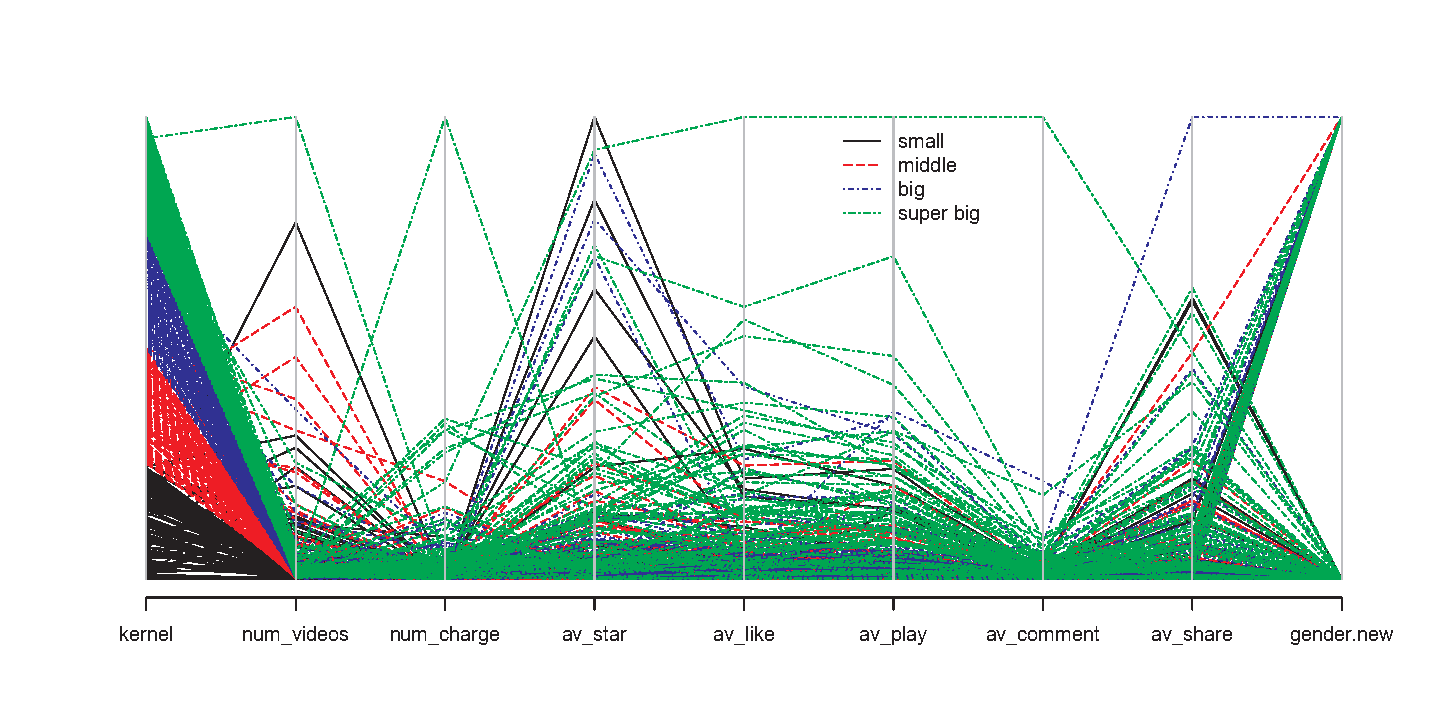
\includegraphics[width=1.0\textwidth]{MLR/Figure_parcoord.png}
    \caption{并行坐标图}
\end{figure}

\subsection{建立模型}

由于响应变量Y是ordinal的,记响应变量fans\_cat为Y,四个粉丝量级与Y的对应关系为:
small(Y=1)<middle(Y=2)<big(Y=3)<super big(Y=4),我们对各水平的累积概率的logit
采用相同的斜率,即采用“平行”的累积逻辑回归模型,模型如下:
\begin{equation}
    \operatorname{logit}(P(Y\le j))=\alpha_j+\beta_1x_1+\cdots+\beta_px_p,\ j=1,2,3
\end{equation}


将响应变量和8个解释变量放入R中得到最初模型,其Anova如下图所示,可以看到性别、视频数量和近期视频平均评论数
这3个解释变量对应的系数均不显著。
\begin{figure}[H]
    \centering
    \begin{minipage}[t]{0.48\textwidth}
        \centering
        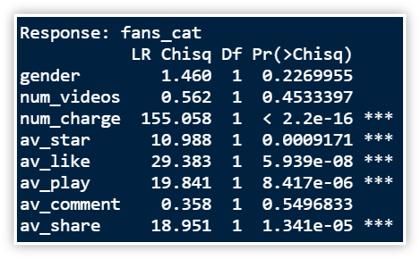
\includegraphics[width=\textwidth]{MLR/Anova1.png}
        \caption{Anova of first model}
    \end{minipage}
    \begin{minipage}[t]{0.48\textwidth}
        \centering
        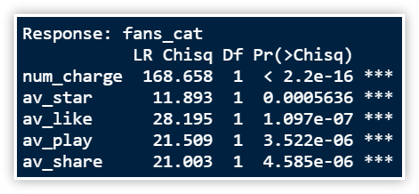
\includegraphics[width=\textwidth]{MLR/Anova2.png}
        \caption{Anova of final model}
    \end{minipage}
\end{figure}


采用Backward Elimination的变量选取方法,并以AIC为准则,可以依次去除近期评论数,
视频数,性别这3个解释变量,将剩余5个解释变量拟合得到最终模型,从图12可以看到
最终模型中5个解释变量均显著。

\subsection{模型解释}

利用R中的vglm函数得到最终的估计模型如下:
\begin{equation*}
    \operatorname{logit}(\hat{P}(Y\le j))=\hat\alpha_j-29.4num\_charge+16.8av\_star-48.6av\_like-19.4av\_play+15.6av\_share
\end{equation*}

其中$\hat\alpha_1=-0.2,\hat\alpha_2=1.3,\hat\alpha_3=2.9$

我们注意到估计模型中$\beta_{num\_charge},\ \beta_{av\_like}, \beta_{av\_play}$均小于0,
说明num\_charge,av\_like,av\_play高的up主更倾向于是量级高的UP主,而
$\beta_{av\_star},\ \beta_{av\_share}$均大于0,说明av\_star和av\_share
高的UP主倾向于是量级低的UP主,这似乎与直觉不太相符,但由于这只是近8个视频的指标,所以
我们可以猜测这些视频可能只是通过“玩梗”等方式在短期获得了较大的关注,或者是新UP主。


结合整个建模过程的分析,我们可以得到以下结论:

(1) 首先性别变量不显著,说明UP主粉丝数量级可能与性别关系不大.

(2) 一些高质量视频的正向收益指标(点赞数,充电数)显著,而总视频数并不显著,
说明相较于视频数量,UP主粉丝数量级与其视频质量的关系更大。说明想成为一名
大Up主,视频在精不在多.

(3) 从拟合模型的系数上看,充电量、点赞量、播放量高的更倾向于是量级高
的UP主,而近期视频收藏量,分享量高的更可能是“昙花一现”。

\subsection{数据可视化}

为了便于数据可视化,我们系数最显著的解释变量充电量num\_charge单独拟合累积逻辑
回归模型得到概率估计图如下,左侧是各个粉丝量级的概率分布,右侧是粉丝数量级的累
积概率。

\begin{figure}[H]
    \centering
    \begin{minipage}[t]{0.48\textwidth}
        \centering
        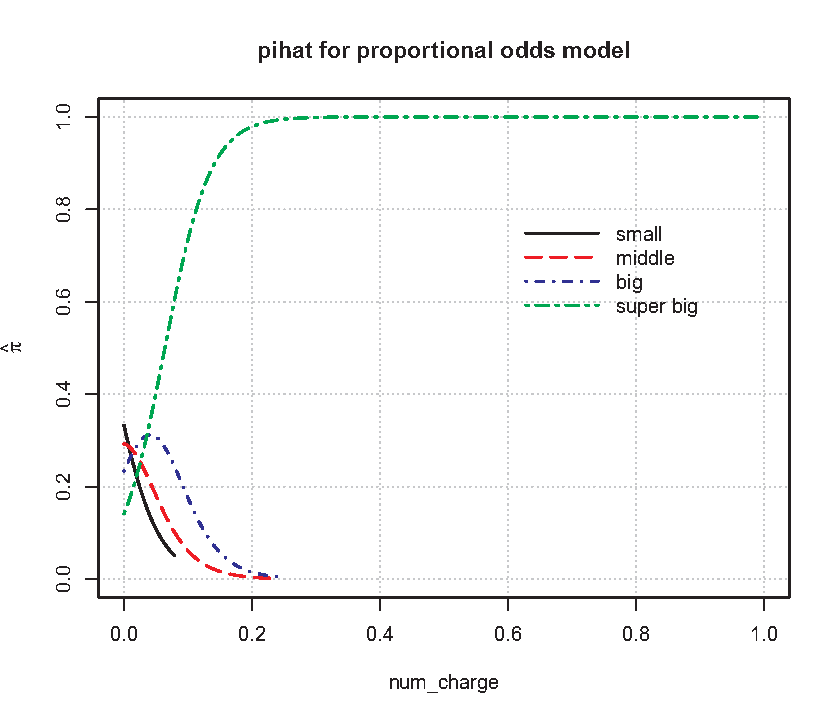
\includegraphics[width=\textwidth]{MLR/Figure_propotional.png}
    \end{minipage}
    \begin{minipage}[t]{0.48\textwidth}
        \centering
        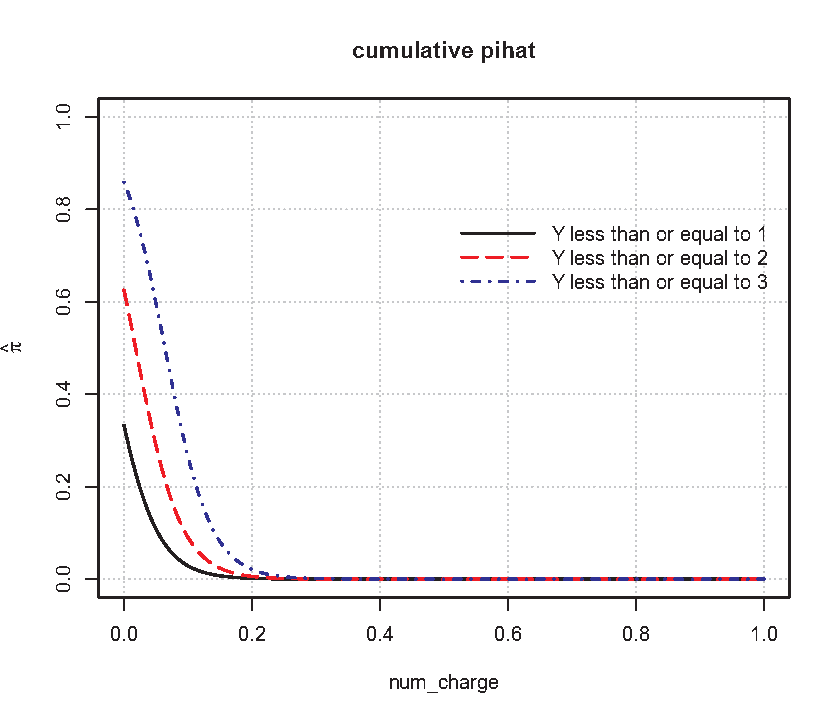
\includegraphics[width=\textwidth]{MLR/Figure_cumulative.png}
        
    \end{minipage}
    \caption{以充电量为解释变量的累积逻辑回归模型概率分布图和累积概率图}
\end{figure}


从左图中我们可以看出充电量在超级大UP主和非超级UP主之间分布非常不均匀,归一化后
的充电量约为0.23以上时,UP主是超级UP主的概率就为1了;从右图可以看出并且随着充
电量的增加,小,中,大量级对应的累积概率都递减,说明充电量稍微大一些,就很可能
是超级UP主了,换言之,归一化后0.23充电量以上的UP主中基本都是超级UP主,这也反映
了一种超级UP主和非超级UP主之间的“贫富差距”大的两极分化现象。

事实上,我们本身抽取UP采用回溯性研究,每个量级的UP主都抽取了250位,但实际上100万
粉以上的超级UP主的数量相较于100万粉以下的小中大UP主的数量是少得可怜的(列联表部分
给出数据),但在抽取数据中充电量23\%值最大值以上都是超级UP主,而充电量本身就是UP主
获得收益的一个主要渠道之一,可见少数的头部UP主获得远多于非头部UP主的收益,这体现了
B站UP主的一种金字塔效应。

\section{研究缺陷与改进}

\subsection{累积逻辑回归模型:“平行”或“非平行”}

在多分类逻辑回归分析部分,我们使用了“平行”的累积回归模型,对于最初的8解释变量
模型,AIC=2273.2;对于最后的5解释变量模型,AIC=2269.1。我们发现最终得到的模型
的AIC依旧在2000以上,说明模型并不是很理想。我们知道,在使用“平行”的累积回归模型
时,我们假定了各解释变量对响应变量各水平的累积变量的影响是一致的,这个假设是否
太强了,导致模型拟合不佳?我们因此尝试了“非平行”的累积逻辑回归模型,当解释变量
为8个时,“非平行”逻辑回归模型的$3\times(8+1)=27$的参数均显著,但是注意到“非平行”
模型的Log-likelihood为NA,经过查阅资料和分析发现,在“非平行”模型情况下出现了累积
概率“交叉”的情况,此时各粉丝量水平概率估计值出现负值,因此导致模型失效,因此“非平
行”模型在本数据中不适用。

\end{document}